%instiki:category: QuantumFieldTheory
\chapter{Three body decays}
\label{cha:three-body-decays} %noinstiki
%instiki:
%instiki:***
%instiki:
%instiki:[[Beyond|Contents]]
%instiki:
%instiki:***
%instiki:
%instiki:* [Muon decay](#mu-decay)
%instiki: 
%instiki:* [three body decays in radiative seesaw](#three-body-decays)
%instiki:
%instiki:* [Sample point](#sample-point)
%instiki:
%instiki:* [Preliminary discussion](#prel-disc)
%instiki:

\section{Muon decay}
\label{sec:mu-decay} 

For a three body decay we have from eq.~\eqref{eq:76}
\begin{align}
  \label{eq:107}
  d\Gamma =& \frac{1}{(2\pi)^5}\frac{1}{2M}\left|\mathcal{M}\right|^2 \delta^4(P-p_1-p_2-p_3)\frac{d^3 p_1}{2E_1}
\frac{d^3 p_2}{2E_2}\frac{d^3 p_3}{2E_3}\nonumber\\
  =& \frac{1}{(2\pi)^5}\frac{1}{2M}\frac{d^3 p_1}{2E_1}\int\left|\mathcal{M}\right|^2 \delta^4(P-p_1-p_2-p_3)
\frac{d^3 p_2}{2E_2}\frac{d^3 p_3}{2E_3}\nonumber\\
\end{align}

\subsection{Amplitude estimation}
\label{sec:amplitude-estimation}
Since $\mathcal{M}$ is dimensionless, the amplitude averaged over spins for $\mu$ decay must be
\begin{equation}
  |\mathcal{M}|^2=C G_F^2 m_\mu^4\,.
\end{equation}
We use
\begin{equation}
  C=\frac{1}{2}(2\times2\times1\times1)=2
\end{equation}
The first factor is for the initial average and the factor are for the number of spin states of $\mu$, $e$ and the two neutrinos. 


Consider first the integral
\begin{align}
  \int \delta^4(P-p_1-p_2)
\frac{d^3 p_1}{2E_1}\frac{d^3 p_2}{2E_2}=&\int\delta(E-E_1-E_2)
\delta^3(\mathbf{P}-\mathbf{p}_1-\mathbf{p}_2)\frac{d^3 p_1}{2E_1}\frac{d^3 p_2}{2E_2}\nonumber\\
  =&\int\delta(E-E_1-E_2)
\frac{d^3 p_2}{4E_1 E_2}\int\delta^3(\mathbf{P}-\mathbf{p}_1-\mathbf{p}_2){d^3 p_1}\nonumber\\
  =&\int\delta(E-E_1-E_2)
\frac{d^3 p_2}{4E_1 E_2}\int\delta^3(\mathbf{p}_1+\mathbf{p}_2-\mathbf{P}){d^3 p_1}\nonumber\\
  =&\int\delta(E-E_1-E_2)
\frac{d^3 p_2}{4E_1 E_2}\int\delta^3[\mathbf{p}_1-(\mathbf{P}-\mathbf{p}_2)]{d^3 p_1}
\end{align}
using
\begin{align}
  \int\delta(x-x_0)dx=1
\end{align}
we have
\begin{align}
  \label{eq:108}
    \int \delta^4(P-p_1-p_2)
\frac{d^3 p_1}{2E_1}\frac{d^3 p_2}{2E_2}=&
\int\delta(E-E_1-E_2)\frac{d^3 p_2}{4E_1 E_2}\nonumber\\
    \int \delta^4(P-p_1-p_2)
\frac{d^3 p_1}{2E_1}\frac{d^3 p_2}{2E_2}=&
\int\delta(E-E_1-E_2)\frac{\mathbf{p}_2^2\,d|\mathbf{p}_2|d\Omega}{4E_1 E_2}
\end{align}
Since $|\mathbf{p}_1|=|\mathbf{p}_2|$ we have
\begin{align}
  E=E_1+E_2=&(m_1^2+\mathbf{p}_1^2)^{1/2}+(m_2^2+\mathbf{p}_2^2)^{1/2}\nonumber\\
  =&(m_1^2+\mathbf{p}_2^2)^{1/2}+(m_2^2+\mathbf{p}_2^2)^{1/2}
\end{align}
differentiating this equation with respect to $\mathbf{p}_2$
\begin{align}
  \frac{d E}{d|\mathbf{p}_2|}=&\frac{1}{2}\left(
\frac{2|\mathbf{p}_2|}{(m_1^2+\mathbf{p}_2^2)^{1/2}}+
\frac{2|\mathbf{p}_2|}{(m_2^2+\mathbf{p}_2^2)^{1/2}}\right)\nonumber\\
=&|\mathbf{p}_2|\left(\frac{1}{E_1}+\frac{1}{E_2}\right)\nonumber\\
  =&|\mathbf{p}_2|\left(\frac{E_1+E_2}{E_1 E_2}\right)
\end{align} 
Therefore
\begin{align}
  d|\mathbf{p}_2|=\frac{d E}{|\mathbf{p}_2|}\left(\frac{E_1 E_2}{E_1+E_2}\right)
\end{align}
replacing back in eq.~(\ref{eq:108})
\begin{align}
      \int \delta^4(P-p_1-p_2)\frac{d^3 p_1}{2E_1}\frac{d^3 p_2}{2E_2}
      =&\int\frac{d E}{|\mathbf{p}_2|}\,\delta(E-E_1-E_2)\frac{\mathbf{p}_2^2\,d\Omega}{4E_1 E_2}
      \left(\frac{E_1 E_2}{E_1+E_2}\right)\nonumber\\
      =&\int d E\,\delta(E-E_1-E_2)\frac{|\mathbf{p}_2|\,d\Omega}{4(E_1+E_2)}\nonumber\\
      =&  \int\frac{|\mathbf{p}_2|}{4 E}d\Omega
\end{align}
For a relativistic particle $|\mathbf{p}_2|\approx E_2=E/2$ and
\begin{align}
  \int \delta^4(P-p_1-p_2)\frac{d^3 p_1}{E_1}\frac{d^3 p_2}{E_2}=2\pi
\end{align}
Applying this result to eq.~(\ref{eq:107}) we have
\begin{align}
    d\Gamma =& \frac{1}{(2\pi)^5}\frac{1}{2M}\frac{d^3 p_1}{2E_1}\int\left|\mathcal{M}\right|^2 \delta^4(P-p_1-p_2-p_3)
\frac{d^3 p_2}{2E_2}\frac{d^3 p_3}{2E_3}\nonumber\\
=&\frac{1}{(2\pi)^5}\frac{1}{2M}\frac{d^3 p_1}{8E_1}\left|\mathcal{M}\right|^2\int \delta^4(P-p_1-p_2-p_3)
\frac{d^3 p_2}{E_2}\frac{d^3 p_3}{E_3}\nonumber\\
=&\frac{1}{(2\pi)^5}\frac{1}{2M}\frac{d^3 p_1}{8E_1}\left|\mathcal{M}\right|^2(2\pi)\nonumber\\
  =&\frac{G_F^2m_\mu^4}{8(2\pi)^4 m_\mu E_1} \mathbf{p}_1^2 d|\mathbf{p}_1|\int d\Omega\nonumber\\
  \approx&\frac{G_F^2m_\mu^3}{8(2\pi)^4  E_1} E_1^2 d E_1(4\pi)\nonumber\\
  \approx&\frac{G_F^2m_\mu^3}{4(2\pi)^3} E_1 d E_1
\end{align}
As the maximum value  of $E_1$ is $m_\mu/2$
\begin{align}
  \Gamma\approx&\frac{G_F^2m_\mu^3}{4(2\pi)^3} \int_0^{m_\mu/2}E_1 d E_1\nonumber\\
   =&\frac{G_F^2m_\mu^3}{4(2\pi)^3} \frac{m_\mu^2}{8}\,,
\end{align}
or
\begin{equation}
  \Gamma=\frac{3}{4}\frac{G_F^2m_\mu^5}{192\pi^3}\,.
\end{equation}

\subsection{Amplitude calculation}
\label{sec:ampl-calc}
The Standard Model Lagrangian includes
\begin{align}
  \mathcal{L}=&-\frac{\sqrt{2}g}{2}(\overline{\nu_e}_L\gamma^\mu e_L W_\mu^++\bar{e}_L\gamma^\mu{\nu_e}_L W_\mu^-+\overline{\nu_\mu}_L\gamma^\mu\mu_L W_\mu^++\bar{\mu}_L\gamma^\mu{\nu_\mu}_L W_\mu^-)\nonumber\\
=&-\frac{g}{\sqrt{2}}(\overline{\nu_e}\gamma^\mu P_L e W_\mu^++\bar{e}\gamma^\mu P_L{\nu_e} W_\mu^-+\overline{\nu_\mu}\gamma^\mu P_L\mu W_\mu^++\bar{\mu}\gamma^\mu P_L{\nu_\mu} W_\mu^-)\nonumber\\
=&-\frac{g}{2\sqrt{2}}(\overline{\nu_e}\gamma^\mu (1-\gamma_5) e W_\mu^++\bar{e}\gamma^\mu (1-\gamma_5){\nu_e} W_\mu^-+\overline{\nu_\mu}\gamma^\mu (1-\gamma_5)\mu W_\mu^++\bar{\mu}\gamma^\mu (1-\gamma_5){\nu_\mu} W_\mu^-)
\end{align}
where
\begin{align}
  \label{eq:109}
  (\overline{\nu_e}\gamma^\mu P_L e W_\mu^+)^\dagger&=e^\dagger{\gamma^\mu P_L}^\dagger(\overline{\nu_e})^\dagger W_\mu^-
  =e^\dagger P_L{\gamma^\mu}^\dagger\gamma^0\nu_e W_\mu^-=e^\dagger\gamma^0\gamma^0{\gamma^\mu}^\dagger P_R\gamma^0\nu_e W_\mu^-\nonumber\\
  &=\bar{e}\gamma^0{\gamma^\mu}^\dagger\gamma^0P_L\nu_e W_\mu^-=\bar{e}\gamma^\mu P_L\nu_e W_\mu^-
\end{align}
We can build the effective Lagrangian

Applying the Feynman rules to the diagram in fig. 
\ref{fig:1} %noinstiki
we have the amplitude
\begin{align}
  \mathcal{M}=\frac{-ig^2}{8}\bar{u}_3\gamma_\mu(1-\gamma_5)u_1\left(\frac{-g^{\mu\nu}+q^\mu q^\nu/M_W^2}{q^2-M_W^2}\right)\bar{u}_4\gamma_\nu(1-\gamma_5)v_2
\end{align}
where $u$ ($v$) is for an incoming particle and $\bar{u}$ ($\bar{v}$) is for an ongoing particle (antiparticle).

\begin{figure} %noinstiki
  \centering %noinstiki
  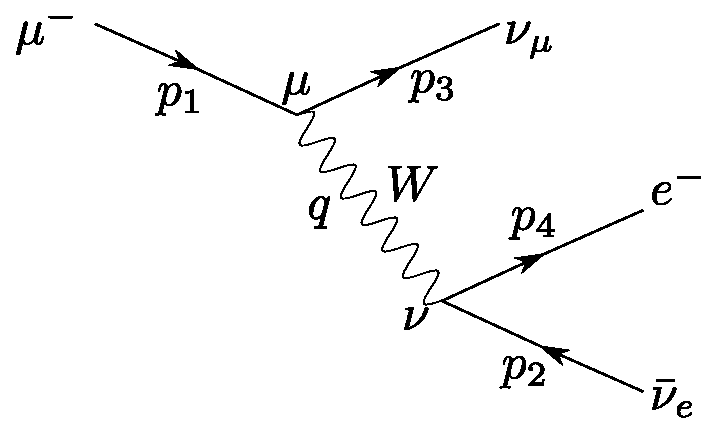
\includegraphics{muon_decay}%noinstiki
  \caption{Tree level diagram for muon decay } %noinstiki
  \label{fig:1} %noinstiki
\end{figure} %noinstiki


The Dirac equations for spinors $u$ and $v$ are
\begin{align}
  (\cancel{p}-m)u&=0&(\cancel{p}+m )v&=0\nonumber\\
  \bar{u}(\cancel{p}-m)&=0&\bar{v}(\cancel{p}+m )&=0\,.
\end{align}
In this way
\begin{align}
  \frac{1}{M_W^2}\gamma_\mu q^\mu(1-\gamma_5)u_1 \bar{u}_4\gamma_\nu q^\nu(1-\gamma_5)
  =&\frac{1}{M_W^2}(1+\gamma_5)\cancel{q}u_1 \bar{u}_4\cancel{q}(1-\gamma_5)\nonumber\\
  =&-\frac{m_\mu m_e}{M_W^2}(1+\gamma_5)u_1 \bar{u}_4(1-\gamma_5)\,
\end{align}
the term in $q^\mu q^\nu$ can be safely neglected. The term $q^2$ is $m_\mu^2$ is small compared with $m_W^2$. Therefore
\begin{align}
  \mathcal{M}=&\frac{-i g^2}{8M_W^2}\bar{u}_3\gamma_\mu(1-\gamma_5)u_1\bar{u}_4\gamma^\mu(1-\gamma_5)v_2\nonumber\\
  =&\frac{-i G_F}{\sqrt{2}}\bar{u}_3\gamma_\mu(1-\gamma_5)u_1\bar{u}_4\gamma^\mu(1-\gamma_5)v_2
\end{align}
$\mathcal{M}$ is a dimensionless scalar. The relevant coupling is
\begin{equation}
  \frac{g^2}{8M_W^2}=\frac{G_F}{\sqrt{2}}\,.
\end{equation}
The conjugate is, following  the same steps that in eq.~\eqref{eq:109}
\begin{align}
  \mathcal{M}^*=&\frac{i g^2}{8M_W^2}\left[\bar{u}_3\gamma_\mu(1-\gamma_5)u_1\right]^\dagger
  \left[\bar{u}_4\gamma^\mu(1-\gamma_5)v_2\right]^\dagger\nonumber\\
   \mathcal{M}^*=&\frac{i g^2}{8M_W^2}\left[\bar{u}_1\gamma_\mu(1-\gamma_5)u_3\right]
  \left[\bar{v}_2\gamma^\mu(1-\gamma_5)u_4\right]\,.
\end{align}
Multiplying $\mathcal{M}$ and $\mathcal{M}^*$ we have
\begin{align}
  \label{eq:110}
  |\mathcal{M}|^2=&\frac{g^4}{64 M_W^4}\left[\bar{u}_3\gamma_\mu(1-\gamma_5)u_1\bar{u}_1\gamma_\nu(1-\gamma_5)u_3\right]\nonumber\\
  &\times\left[\bar{u}_4\gamma^\mu(1-\gamma_5)v_2\bar{v}_2\gamma^\nu(1-\gamma_5)u_4\right]\nonumber\\
  =&\frac{g^4}{64 M_W^4}L_{\mu\nu}M^{\mu\nu}
\end{align}
where
\begin{align}
   L_{\mu\nu}=&\left[\bar{u}_{3\alpha}\gamma_\mu^{\alpha\beta}(1-\gamma_5)_{\beta\gamma}u_1^\gamma\bar{u}_{1\delta}\gamma_\nu^{\delta\epsilon}(1-\gamma_5)_{\epsilon\eta}u_3^\eta\right]\nonumber\\
  M^{\mu\nu}=&\left[\bar{u}_4^\alpha\gamma^\mu_{\alpha\beta}(1-\gamma_5)^{\beta\gamma}v_{2\gamma}\bar{v}_2^\delta\gamma^\nu_{\delta\epsilon}(1-\gamma_5)^{\epsilon\eta}u_{4\eta}\right]
\end{align}
\begin{align}
     L_{\mu\nu}=&\left[u_3^\eta\bar{u}_{3\alpha}\gamma_\mu^{\alpha\beta}(1-\gamma_5)_{\beta\gamma}u_1^\gamma\bar{u}_{1\delta}\gamma_\nu^{\delta\epsilon}(1-\gamma_5)_{\epsilon\eta}\right]\nonumber\\
     =&\left[(u_3\bar{u}_{3})_{\eta\alpha}\gamma_\mu^{\alpha\beta}(1-\gamma_5)_{\beta\gamma}(u_1\bar{u}_{1})_{\gamma\delta}\gamma_\nu^{\delta\epsilon}(1-\gamma_5)_{\epsilon\eta}\right]\nonumber\\
     =&\operatorname{Tr}\left[(u_3\bar{u}_{3})\gamma_\mu(1-\gamma_5)(u_1\bar{u}_{1})\gamma_\nu(1-\gamma_5)\right]
\end{align}
Using
\begin{align}
  \label{eq:111}
 \sum_su(p,s)\bar{u}(p,s)&=(\cancel{p}+m)& \sum_sv(p,s)\bar{v}(p,s)&=(\cancel{p}-m)
\end{align}
\begin{align}
  \sum_s L_{\mu\nu}=&\operatorname{Tr}\left[(\cancel{p}_3)\gamma_\mu(1-\gamma_5)(\cancel{p}_1+m_\mu)\gamma_\nu(1-\gamma_5)\right]\nonumber\\
  =&p_3^\alpha\operatorname{Tr}\left[\gamma_\alpha\gamma_\mu(1-\gamma_5)(p_1^\beta\gamma_\beta+m_\mu)\gamma_\nu(1-\gamma_5)\right]\nonumber\\
  =&p_3^\alpha\operatorname{Tr}\left[(\gamma_\alpha\gamma_\mu-\gamma_\alpha\gamma_\mu\gamma_5)(p_1^\beta\gamma_\beta\gamma_\nu(1-\gamma_5)+m_\mu\gamma_\nu(1-\gamma_5))\right]\nonumber\\
  =&p_3^\alpha\operatorname{Tr}\left[p_1^\beta\gamma_\alpha\gamma_\mu\gamma_\beta\gamma_\nu(1-\gamma_5)-p_1^\beta\gamma_\alpha\gamma_\mu\gamma_5\gamma_\beta\gamma_\nu(1-\gamma_5)\right.\nonumber\\
&\left.+m_\mu\gamma_\alpha\gamma_\mu\gamma_\nu(1-\gamma_5)-m_\mu\gamma_\alpha\gamma_\mu\gamma_5\gamma_\nu(1-\gamma_5)\right]\nonumber\\
  =&p_3^\alpha\operatorname{Tr}\left[p_1^\beta\gamma_\alpha\gamma_\mu\gamma_\beta\gamma_\nu-p_1^\beta\gamma_\alpha\gamma_\mu\gamma_\beta\gamma_\nu\gamma_5-p_1^\beta\gamma_\alpha\gamma_\mu\gamma_5\gamma_\beta\gamma_\nu
+p_1^\beta\gamma_\alpha\gamma_\mu\gamma_5\gamma_\beta\gamma_\nu\gamma_5\right.\nonumber\\
&\left.+m_\mu\gamma_\alpha\gamma_\mu\gamma_\nu-m_\mu\gamma_\alpha\gamma_\mu\gamma_\nu\gamma_5-m_\mu\gamma_\alpha\gamma_\mu\gamma_5\gamma_\nu+m_\mu\gamma_\alpha\gamma_\mu\gamma_5\gamma_\nu\gamma_5\right]
\end{align}
as the trace of an odd number of $\gamma$--matrices is zero, we have
\begin{align}
  \sum_s L_{\mu\nu}=&p_3^\alpha p_1^\beta\operatorname{Tr}\left[\gamma_\alpha\gamma_\mu\gamma_\beta\gamma_\nu-\gamma_\alpha\gamma_\mu\gamma_\beta\gamma_\nu\gamma_5-\gamma_\alpha\gamma_\mu\gamma_\beta\gamma_\nu\gamma_5
+\gamma_\alpha\gamma_\mu\gamma_\beta\gamma_\nu\gamma_5^2\right]\nonumber\\
=&2 p_3^\alpha p_1^\beta\operatorname{Tr}\left[\gamma_\alpha\gamma_\mu\gamma_\beta\gamma_\nu(1-\gamma_5)\right]
\end{align}
Similarly
\begin{align}
  \sum_s M^{\mu\nu}=2 p_{4\delta}p_{2\epsilon}\operatorname{Tr}\left[\gamma^\delta\gamma^\mu\gamma^\epsilon\gamma^\nu(1-\gamma_5)\right]
\end{align}
substituting back in eq.~(\ref{eq:110}) we have,
\begin{align}
  \label{eq:112}
   |\mathcal{M}|^2=&\frac{g^4}{64 M_W^4}4p_3^\alpha p_1^\beta p_{4\delta}p_{2\epsilon}
   \operatorname{Tr}\left[\gamma_\alpha\gamma_\mu\gamma_\beta\gamma_\nu(1-\gamma_5)\right]
   \operatorname{Tr}\left[\gamma^\delta\gamma^\mu\gamma^\epsilon\gamma^\nu(1-\gamma_5)\right]\nonumber\\
   =&\frac{g^4}{64 M_W^4}4p_3^\alpha p_1^\beta p_{4\delta}p_{2\epsilon}(64\delta^\alpha_\delta\delta^\beta_\epsilon)\nonumber\\
  =&\frac{g^4}{64 M_W^4}4\times64(p_3\cdot p_4)(p_1\cdot p_2)\nonumber\\
  =&\frac{4g^4}{M_W^4}(p_3\cdot p_4)(p_1\cdot p_2)\nonumber\\
  =&4\left(8\frac{g^2}{8M_W^2}\right)^2(p_3\cdot p_4)(p_1\cdot p_2)\nonumber\\
  =&4\left(8\frac{G_F}{\sqrt{2}}\right)^2(p_3\cdot p_4)(p_1\cdot p_2)\nonumber\\
  =&128\, G_F^2(p_3\cdot p_4)(p_1\cdot p_2)\nonumber\\
  =&256\frac{G_F^2}{{2}}(p_3\cdot p_4)(p_1\cdot p_2)\,.
\end{align}
The demonstration of the used Tr$\times$Tr identity can be found in Appendix B. of \cite{PeterRenton}.

The spin--averaged differential decay width for $\mu^-\to\nu_\mu e^-\bar{\nu}_e$ is
\begin{align}
  \label{eq:113}
  d\Gamma =& \frac{1}{(2\pi)^5}\frac{1}{2E_1}\frac{d^3 p_3}{2E_3}
\left(\frac{1}{2}\sum\left|\mathcal{M}\right|^2\right) \delta^4(p_1-p_2-p_3-p_4)
\frac{d^3 p_2}{2E_2}\frac{d^3 p_4}{2E_4}\nonumber\\
 =&\frac{1}{2E_1}\frac{1}{2}\sum\left|\mathcal{M}\right|^2\frac{1}{(2\pi)^5}\frac{d^3 p_2}{8E_2}
  \delta^4(p_1-p_2-p_3-p_4)\frac{d^3 p_3}{E_3}\frac{d^3 p_4}{E_4}\nonumber\\
=&\frac{1}{2}\frac{4g^4}{M_W^4}\frac{1}{(2\pi)^52E_1}(p_1\cdot p_2)(p_3\cdot p_4)\frac{d^3 p_2}{2E_2}
  \delta^4(p_1-p_2-p_3-p_4)\frac{d^3 p_3}{2E_3}\frac{d^3 p_4}{2E_4}\nonumber\\
  =&\frac{2g^4}{16 (2\pi)^5 M_W^4 E_1 E_4}p_1^\beta p_4^\alpha d^3p_4 I_{\alpha\beta}
\end{align}
where the covariant integral $I_{\alpha\beta}$ on the neutrino momentum is
\begin{align}
  \label{eq:114}
  I_{\alpha\beta}=\int p_{3\alpha}p_{2\beta}\delta^4(p-p_2-p_3)\frac{d^3 p_2}{E_2}\frac{d^3 p_3}{E_3}\,.
\end{align}
The variable $p$ in ec.~\eqref{eq:114} is defined as $p=p_1-p_4=p_2+p_3$. Moreover
\begin{align}
  \label{eq:115}
  p^2=&p_2^2+p_3^2+2p_2\cdot p_3\nonumber\\
  =&m_{\nu_e}^2+m_{\nu_\mu}^2+2p_2\cdot p_3\nonumber\\
  \approx&2p_2\cdot p_3\nonumber\\
g_{\alpha\beta}p^\alpha p^\beta=&2 g_{\alpha\beta}p_3^\alpha p_2^\beta\nonumber\\
p^\alpha p^\beta=&2p_3^\alpha p_2^\beta\,.
\end{align}
$I_{\alpha\beta}$ must have the form
\begin{align}
  \label{eq:116}
  I_{\alpha\beta}=g_{\alpha\beta}A(p^2)+p_\alpha p_\beta B(p^2)\,.
\end{align}
Defining the itegral $I$ as follows
\begin{equation}
  I=\int\delta^4(p-p_2-p_3)\frac{d^3 p_2}{E_2}\frac{d^3 p_3}{E_3}\,,
\end{equation}
Since
\begin{align}
  m_\nu^2\approx0=&E_\nu^2-\mathbf{p}_\nu^2\nonumber\\
E_\nu^2=&\mathbf{p}_\nu^2
\end{align}
and in addition the integral $I$ is covariant, we choose to evaluate it in the rest frame of the two neutrinos
$|\mathbf{p}_2|=|\mathbf{p}_3|$, which implies $E_2=E_3$.
\begin{align}
  I=&\int\delta(E-E_2-E_3)\delta^3(\mathbf{p}-\mathbf{p}_2-\mathbf{p}_3)\frac{d^3 p_2}{E_2}\frac{d^3 p_3}{E_3}\nonumber\\
    =&\int\delta(E-E_2-E_3)\frac{d^3 p_2}{E_2E_3}\underbrace{\int\delta^3(\mathbf{p}-\mathbf{p}_2-\mathbf{p}_3)d^3 p_3}_{=1}\nonumber\\
    =&\int\frac{\delta(E-2E_2)}{E_2^2}\mathbf{p}_2^2 d|\mathbf{p}_2|d\Omega\nonumber\\
    =&\int\frac{\delta(E-2E_2)}{E_2^2}E_2^2 dE_2 (4\pi)\nonumber\\
    =&4\pi\int\delta\left(2\left(E_2-\frac{E}{2}\right)\right) dE_2 \nonumber\\
    =&4\pi\frac{1}{2}\int\delta\left(E_2-\frac{E}{2}\right) dE_2 \nonumber\\
    =&2\pi
\end{align}

then multiplying (6.13) by $g^{\alpha\beta}$ and $p^\alpha p^\beta$ successively gives, using eq.~\eqref{eq:115}
\begin{equation}
  g^{\alpha\beta}I_{\alpha\beta}=4 A +p^2 B=\int p_{3}\cdot
  p_{2}\delta^4(p-p_2-p_3)\frac{d^3 p_2}{E_2}\frac{d^3
    p_3}{E_3}\nonumber =\frac{p^2}{2}I=\pi p^2\nonumber
\end{equation}

In order to compute $p^\alpha p^\beta I_{\alpha\beta}$, we make use of
the fact that it is a Lorentz invariant quantity, so that we may
evaluate it in any reference frame. In particular, we can evaluate it
in the rest frame of the neutrinos involved in this process. This
means that $p=p_2+p_3=(p^0,\mathbf{0})$ and $E_2=E_3$
\begin{align}
p^\alpha p^\beta I_{\alpha\beta}&=p^2 A+p^4 B\\ 
&=p^\alpha
p^\beta\int\frac{d^3 p_2}{E_2}\frac{d^3 p_3}{E_3}
p_{3\alpha}p_{2\beta}\delta^4(p-p_2-p_3) \nonumber\\
&=\int \frac{d^3
  p_2}{E_2}\frac{d^3 p_3}{E_3} E_3p^0E_2p^0\delta^4(p-p_2-p_3)\nonumber\\
&=(p^0)^2\int d^3 p_2d^3 p_3
\delta^4(p-p_2-p_3)\\
&=(p^0)^2\int d^3 p_2 \delta(p^0-2E_2)\nonumber\\
&=(p)^2\int d E_2 E_2^2 d\Omega
\frac{1}{2}\delta(\frac{p^0}{2}-E_2) 
=4\pi\frac{p^2}{2}\left(\frac{p^2}{2}\right)^2 \nonumber\\
&=\frac{\pi p^4}{2}
\end{align}
where the usual tricks have been used to simplify the integrals, using
the delta function inside.

Therefore
\begin{equation}
  A=\frac{p^2}{4}(\pi-B)
\end{equation}
\begin{align}
  \frac{p^4}{4}(\pi-B)+p^4B=&\frac{\pi p^4}{2}\nonumber\\
    \frac{\pi}{4} -\frac{B}{4}+B=&\frac{\pi}{2}\nonumber\\
    \frac{3B}{4}=&\frac{\pi}{4}\nonumber\\
    B=&\frac{\pi}{3}
\end{align}
\begin{align}
  A=&\frac{p^2}{4}(\pi-\frac{\pi}{3})\nonumber\\
  =&\frac{p^2}{4}(\frac{2\pi}{3})\nonumber\\
  =&\frac{\pi p^2}{6}
\end{align}
\begin{align}
  I_{\alpha\beta}=\frac{\pi}{6}\left(g_{\alpha\beta}p^2+2p_\alpha p_\beta  \right)\,.
\end{align}
Substituting back in eq.~(\ref{eq:113}) we have 
\begin{align}
  \label{eq:117}
  d\Gamma =& \frac{2\pi g^4}{16\times6 (2\pi)^5 M_W^4 E_1 E_4}p_1^\beta p_4^\alpha (g_{\alpha\beta}p^2+2p_\alpha p_\beta)d^3p_4 \nonumber\\
  d\Gamma =& \frac{2g^4}{16\times12 (2\pi)^4 M_W^4 E_1 E_4}[(p_1\cdot p_4)p^2+2(p\cdot p_1)(p\cdot p_4)]d^3p_4 \nonumber\\
  d\Gamma =& \frac{2g^4}{192 (2\pi)^4 M_W^4 E_1 E_4}[(p_1\cdot p_4)p^2+2(p\cdot p_1)(p\cdot p_4)]d^3p_4 
\end{align}
For further evaluation we will use the rest frame of the decaying muon. In this frame the four--momentum are
\begin{align}
  p_1=&(m_\mu,\mathbf{0})\nonumber\\
  p_4=&(E_4,\mathbf{p}_4)\nonumber\\
  p=&p_1-p_4=(m_\mu-E_4,-\mathbf{p}_4)\nonumber\\
  p^2=&E^2-\mathbf{p}^2=m_\mu^2-2m_\mu E_4+(E_4^2-\mathbf{p}_4^2)=m_\mu^2+m_e^2-2m_\mu E_4
\end{align}
Moreover
\begin{align}
  \label{eq:118}
  p_1\cdot p_4=&m_\mu E_4\nonumber\\
  p\cdot p_1=&m_\mu^2-m_\mu E_4\nonumber\\
  p\cdot p_4=&m_\mu E_4-E_4^2+\mathbf{p}_4^2=m_\mu E_4-m_e^2\nonumber\\
  p_4^2=m_e^2&=E_4^2-\mathbf{p}_4^2\Rightarrow\mathbf{p}_4^2=E_4^2-m_e^2\nonumber\\
  |\mathbf{p}_4| =&(E_4^2-m_e^2)^{1/2}\nonumber\\
  &\Rightarrow\frac{d|\mathbf{p}_4|}{d E_4}=\frac{1}{2}\frac{2E_4}{(E_4^2-m_e^2)^{1/2}}=\frac{E_4}{|\mathbf{p}_4|}\nonumber\\
  &\Rightarrow d|\mathbf{p}_4|=\frac{E_4}{|\mathbf{p}_4|} d E_4\nonumber\\
  d^3p_4=&\mathbf{p}_4^2 \,d |\mathbf{p}_4|\,d\Omega=|\mathbf{p}_4|E_4\,d E_4\, d\Omega
\end{align}
Substituting back in eq.~(\ref{eq:117}) we have 
\begin{align}
  d\Gamma=&\frac{2g^4}{192 (2\pi)^4 M_W^4 m_\mu }|\mathbf{p}_4|\,d E_4\,d\Omega[(m_\mu^2+m_e^2-2m_\mu E_4)m_\mu E_4 
  +2(m_\mu^2-m_\mu E_4)(m_\mu E_4-m_e^2)]
\end{align}
Neglecting electron mass we have $|\mathbf{p}_4| = E_4$, and
\begin{align}
   d\Gamma=&\frac{2g^4(4\pi)}{192 (2\pi)^4 M_W^4 m_\mu }E_4\,d E_4[(m_\mu^2-2m_\mu E_4)m_\mu E_4 
  +2(m_\mu^2-m_\mu E_4)m_\mu E_4]\nonumber\\
  =&\frac{2\times2g^4}{192 (2\pi)^3 M_W^4 m_\mu }m_\mu E_4^2[m_\mu^2-2m_\mu E_4
  +2m_\mu^2-2m_\mu E_4]\,d E_4\nonumber\\
  =&\frac{4g^4}{192 (2\pi)^3 M_W^4 }E_4^2\left[3m_\mu^2-4m_\mu E_4\right]\,d E_4\nonumber\\
  =&\frac{4g^4}{192 (2\pi)^3 M_W^4 }m_\mu^2E_4^2\left[3-4\frac{E_4}{m_\mu}\right]\,d E_4\nonumber\\
  =&\frac{4g^4}{192 (2\pi)^3 M_W^4 }\frac{m_\mu^4}{4}\left(\frac{2E_4}{m_\mu}\right)^2
  \left[3-2\left(\frac{2E_4}{m_\mu}\right)\right]\frac{m_\mu}{2}\,d \left(\frac{2E_4}{m_\mu}\right)\nonumber\\
 =&\frac{4g^4}{192 (2\pi)^3 M_W^4 }\frac{m_\mu^5}{8}\left(\frac{2E_4}{m_\mu}\right)^2
  \left[3-2\left(\frac{2E_4}{m_\mu}\right)\right]\,d \left(\frac{2E_4}{m_\mu}\right)
\end{align}
$E_4$ varies from 0 to $E_4^{\text{max}}$ can be obtained from ($m_e=0)$
\begin{align}
  \label{eq:119}
p_1-p_4=p_2+p_3\,.
\end{align}
The square of he factor on the left is
\begin{align}
  (p_1-p_4)^2=&p_1^2+p_4^2-2p_1\cdot p_4\nonumber\\
  =&m_\mu^2+m_e^2-2p_1\cdot p_4\,.
\end{align}
We have then using eqs.~(\ref{eq:118})(\ref{eq:119})
\begin{align}
  2p_1\cdot p_4=&m_\mu^2+m_e^2-(p_1+p_4)^2\nonumber\\
  2m_\mu E_4=&m_\mu^2+m_e^2-(p_2+p_3)^2\nonumber\\
  \approx&m_\mu^2-(p_2+p_3)^2\,.
\end{align}
$(p_2+p_3)^2$ is the invariant mass squared of the $\nu_\mu+\bar{\nu}_e$ system, which ranges from $0$ to $m_\mu^2$. For $(p_2+p_3)^2=m_\mu$ we have $E_4^{\text{min}}=0$, while for $(p_2+p_3)^2=0$ we have $E_4^{\text{max}}=m_\mu/2$. The missing integration on $d\Gamma$ is in the variable $x$ such that
\begin{equation}
  x=\frac{2E}{m_\mu}\,,\qquad x_{\text{min}}=0\,,\qquad x_{\text{max}}=\frac{2E_{\text{max}}}{m_\mu}=1\,.
\end{equation}
Therefore

\begin{align}
  \Gamma=&\frac{4g^4}{192 (2\pi)^3 M_W^4 }\frac{m_\mu^5}{8}\int_0^1x^2[3-2x]\,d x\nonumber\\
  =&\frac{4g^4}{192 (2\pi)^3 M_W^4 }\frac{m_\mu^5}{8}\frac{1}{2}\nonumber\\
  =&\frac{g^4}{192 \pi^3 8M_W^4 }\frac{m_\mu^5}{4}\nonumber\\
  =&\frac{g^4}{64 M_W^4 }\frac{2}{192 \pi^3}m_\mu^5\nonumber\\
  =&\frac{G_F^2}{2}\frac{2}{192 \pi^3}m_\mu^5\nonumber\\
  =&\frac{G_F^2}{192 \pi^3}m_\mu^5
\end{align}
Without neglect the electron mass we have
\begin{align}
  d\Gamma=&\frac{2g^4}{192 (2\pi)^4 M_W^4 m_\mu }|\mathbf{p}_4|\,d E_4\,d\Omega[(m_\mu^2+m_e^2-2m_\mu E_4)m_\mu E_4 
  +2(m_\mu^2-m_\mu E_4)(m_\mu E_4-m_e^2)]\nonumber\\
  =&\frac{4g^4}{192 (2\pi)^3 M_W^4 m_\mu }\,d E_4(E_4^2-m_e^2)^{1/2}[m_\mu^3 E_4+m_e^2m_\mu E_4-2(m_\mu E_4)^2 \nonumber\\
  &+2m_\mu^3 E_4-2(m_\mu E_4)^2-2m_\mu^2m_e^2+2m_\mu m_e^2 E_4]\nonumber\\
 d\Gamma =&\frac{4g^4}{192 (2\pi)^3 M_W^4 m_\mu }\,d E_4(E_4^2-m_e^2)^{1/2}[3m_\mu^3 E_4+3 m_e^2m_\mu E_4-4(m_\mu E_4)^2 
  -2m_\mu^2m_e^2]
\end{align}
The decay width, in terms of $x=m_e/m_\mu$ is
\begin{align}
  \label{eq:120}
 \Gamma =&\frac{4g^4}{192 (2\pi)^3 M_W^4 m_\mu }\int_{m_e}^{m_\mu(1+x^2)/2}(E_4^2-m_e^2)^{1/2}[(3m_\mu^2+3 m_e^2-4m_\mu E_4)m_\mu E_4
  -2m_\mu^2m_e^2]\,d E_4\nonumber\\
=&\frac{4g^4}{192 (2\pi)^3 M_W^4 m_\mu }\frac{m_\mu^6}{16}I\left(x\right)\,,\qquad I(x)=1-8x^2-24x^4\ln(x)+8x^6-x^8\nonumber\\
 =&\frac{G_F^2 m_\mu^5}{192\pi^3}I\left(x\right)\nonumber\\
=&\left(\frac{G_F}{\sqrt{2}}\right)^2\frac{m_\mu^5}{96\pi^3}I\left(x\right)\,,
\end{align}

\section{three body decays in radiative seesaw}
\label{sec:three-body-decays}
We have the Lagrangian \cite{Sierra:2008wj}
\begin{align}
  \mathcal{L}=&\epsilon_{a b}  h_{\alpha j}\overline{N}_j P_L L_\alpha^a \eta^b + \mbox{h.c.}\nonumber\\
  =&h_{\alpha j}\overline{N}_j P_L L_\alpha^1 \eta^2- h_{\alpha j}\overline{N}_j P_L L_\alpha^2 \eta^1+ \mbox{h.c.}\nonumber\\
  =&h_{\alpha j}\overline{N}_j P_L \nu_\alpha \eta^0- h_{\alpha j}\overline{N}_j P_L l_\alpha \eta^++\text{h.c}
\end{align}
where
\begin{align}
  (\overline{N}_j P_L l_\alpha \eta^+)^\dagger=l_\alpha^\dagger P_L\gamma^0N_j\eta^-=\bar{l}_\alpha P_R\gamma^0N_j\eta^-
\end{align}
Therefore
\begin{align}
     \mathcal{L}=&h_{\alpha j}\overline{N}_j P_L \nu_\alpha \eta^0- h_{\alpha j}\overline{N}_j P_L l_\alpha \eta^+
   +h_{\alpha j}^*\overline{\nu}_\alpha P_R N_j \eta^{*0}- h_{\alpha j}^*\overline{l}_\alpha P_R {N}_j \eta^- \nonumber\\
  =&\frac{1}{2}\left[h_{\alpha j}\overline{N}_j (1-\gamma_5) \nu_\alpha \eta^0- h_{\alpha j}\overline{N}_j (1-\gamma_5) l_\alpha \eta^+
   +h_{\alpha j}^*\overline{\nu}_\alpha (1+\gamma_5) N_j \eta^{*0}- h_{\alpha j}^*\overline{l}_\alpha (1+\gamma_5) {N}_j \eta^- \right]
\end{align}
Applying Feynman  rules  to the diagram in fig.2 $N_j(p_1) \to l^-_\alpha(p_3) h^+$, $h^+\to l^+_\beta(p_2)+N_i(p_4)$. 
\begin{figure} %noinstiki
  \centering %noinstiki
  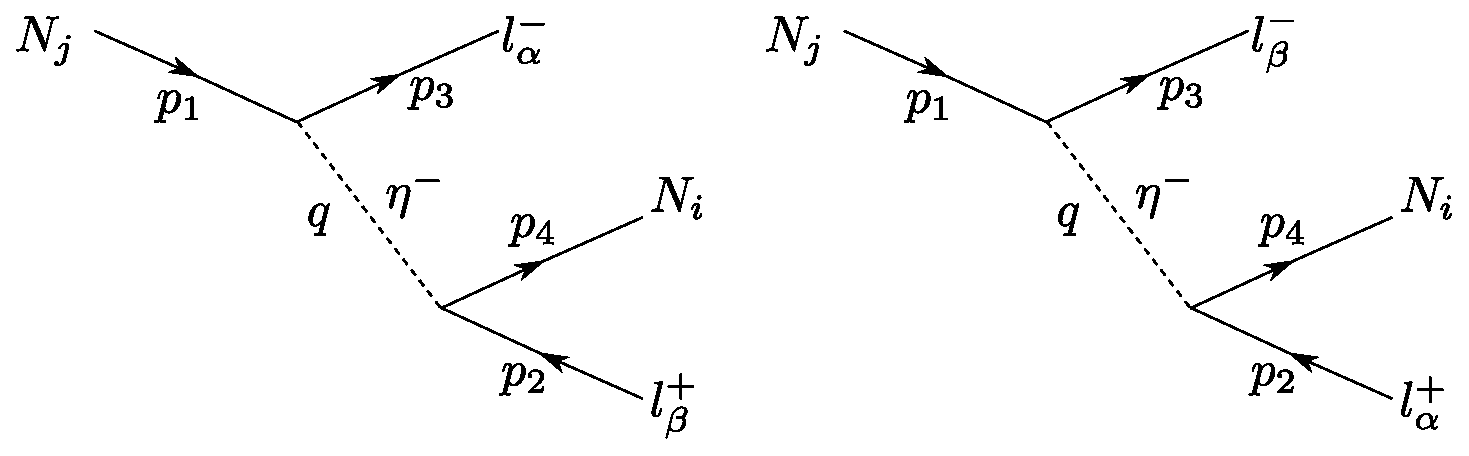
\includegraphics[scale=0.7]{nj_decay} %noinstiki
  \caption{Tree level diagram for $N_j$ decay } %noinstiki
  \label{fig:2} %noinstiki
\end{figure} %noinstiki


we have the amplitude 
\begin{align}
  \mathcal{M}=&-i
  h_{\alpha j}\bar{u}_3(1-\gamma_5)u_1\left(\frac{1}{q^2-M_\eta^2}\right)h_{\beta i}\bar{u}_4(1-\gamma_5)v_2\nonumber\\
  &-i h_{\beta j}\bar{u}_3(1-\gamma_5)u_1\left(\frac{1}{q^2-M_\eta^2}\right)h_{\alpha i}\bar{u}_4(1-\gamma_5)v_2\nonumber\\
  \approx&-\frac{iH_{\alpha\beta ij}}{{M_\eta^2}}\bar{u}_3(1-\gamma_5)u_1\bar{u}_4(1-\gamma_5)v_2
\end{align}
where
\begin{equation}
  H_{\alpha\beta ij}=h_{\alpha j}h_{\beta i}+h_{\alpha i}h_{\beta j}
\end{equation}
\begin{align}
   \mathcal{M}^*=&-\frac{iH_{\alpha\beta ij}}{{M_\eta^2}}
   [\bar{u}_3(1-\gamma_5)u_1]^\dagger[\bar{u}_4(1-\gamma_5)v_2]^\dagger\nonumber\\
   =&-\frac{iH_{\alpha\beta ij}}{{M_\eta^2}}[\bar{u}_1(1+\gamma_5)u_3][\bar{v}_2(1+\gamma_5)u_4]\,.
\end{align}

Multiplying $\mathcal{M}$ and $\mathcal{M}^*$ we have
\begin{align}
\left|\mathcal{M}\right|^2=&\frac{H_{\alpha \beta i j}^2}{M_\eta^4}
[\bar{u}_3^\alpha(1-\gamma_5)_{\alpha\beta}u_1^\beta\bar{u}_1^\gamma(1+\gamma_5)_{\gamma\delta}u_3^\delta]
[\bar{u}_4^\alpha(1-\gamma_5)_{\alpha\beta}v_2^\beta\bar{v}_2^\gamma(1+\gamma_5)_{\gamma\delta}u_4^\delta]\nonumber\\
  =&\frac{H_{\alpha\beta i j}^2}{M_\eta^4}
[u_3^\delta\bar{u}_3^\alpha(1-\gamma_5)_{\alpha\beta}u_1^\beta\bar{u}_1^\gamma(1+\gamma_5)_{\gamma\delta}]
[u_4^\delta\bar{u}_4^\alpha(1-\gamma_5)_{\alpha\beta}v_2^\beta\bar{v}_2^\gamma(1+\gamma_5)_{\gamma\delta}]\nonumber\\
  =&\frac{H_{\alpha\beta i j}^2}{M_\eta^4}
[(u_3\bar{u}_3)_{\delta\alpha}(1-\gamma_5)_{\alpha\beta}(u_1\bar{u}_1)_{\beta\gamma}(1+\gamma_5)_{\gamma\delta}]
[(u_4\bar{u}_4)_{\delta\alpha}(1-\gamma_5)_{\alpha\beta}(v_2\bar{v}_2)_{\beta\gamma}(1+\gamma_5)_{\gamma\delta}]\nonumber\\
=&\frac{H_{\alpha\beta i j}^2}{M_\eta^4}
\operatorname{Tr}[(u_3\bar{u}_3)(1-\gamma_5)(u_1\bar{u}_1)(1+\gamma_5)]
\operatorname{Tr}[(u_4\bar{u}_4)(1-\gamma_5)(v_2\bar{v}_2)(1+\gamma_5)]
\end{align}
Using eq.~\eqref{eq:111}, and neglecting charged fermion masses
\begin{align}
\left|\mathcal{M}\right|^2=&\frac{H_{\alpha\beta i j}^2}{M_\eta^4}
\operatorname{Tr}[\cancel{p}_3(1-\gamma_5)(\cancel{p}_1+M_j)(1+\gamma_5)]
\operatorname{Tr}[(\cancel{p}_4+M_i)(1-\gamma_5)\cancel{p}_2(1+\gamma_5)]\nonumber\\
=&\frac{H_{\alpha\beta i j}^2}{M_\eta^4} L M
\end{align}
\begin{align}
  L=&\operatorname{Tr}[(\cancel{p}_3-\cancel{p}_3\gamma_5)(\cancel{p}_1+\cancel{p}_1\gamma_5+M_j+M_j\gamma_5]
\end{align}
\begin{align}
  L=&\operatorname{Tr}[\cancel{p}_3\cancel{p}_1+\cancel{p}_3\cancel{p}_1\gamma_5+M_j\cancel{p}_3+M_j\cancel{p}_3\gamma_5-\cancel{p}_3\gamma_5\cancel{p}_1-\cancel{p}_3\gamma_5\cancel{p}_1\gamma_5-\cancel{p}_3\gamma_5M_j+M_j\gamma_5]\nonumber\\
  =&2\operatorname{Tr}[\cancel{p}_3\cancel{p}_1]\nonumber\\
  =&2p_3^\alpha p_1^\beta\operatorname{Tr}[\gamma_\alpha\gamma_\beta]\nonumber\\
  =&8p_3^\alpha p_1^\beta g_{\alpha\beta}\nonumber\\
  =&8(p_3\cdot p_1)
\end{align}
Similarly
\begin{align}
  M=8(p_4\cdot p_2)
\end{align}
Therefore
\begin{align}
  \left|\mathcal{M}\right|^2=&\frac{H_{\alpha\beta i j}^2}{M_\eta^4}64(p_3\cdot p_4)(p_1\cdot p_2)\nonumber\\
  \left|\mathcal{M}\right|^2=&\frac{H_{\alpha\beta i j}^2}{4M_\eta^4}4\times64(p_3\cdot p_4)(p_1\cdot p_2)\nonumber\\
\end{align}
In this way, comparing with eq.~\eqref{eq:112}, the results for the moun decay can be directly used after the replacements
\begin{align}
  \frac{g^4}{64 M_W^4}&\to\frac{H_{\alpha\beta i j}^2}{4M_\eta^4}\nonumber\\
  \frac{g^4}{M_W^4}&\to\frac{16H_{\alpha\beta i j}^2}{M_\eta^4}\nonumber\\
  m_\mu&\to M_j\nonumber\\
  x=\frac{m_e}{m_\mu}&\to\frac{M_i}{M_j}\,.
\end{align}
The decay width is according eq.~\eqref{eq:120}
\begin{align}
  \label{eq:121}
  \Gamma(N_j\to l_\alpha^\mp l_\beta^\pm N_i)=&\frac{16H_{\alpha\beta ij}^2}{M_\eta^4}
  \frac{4}{192 (2\pi)^3 M_j }\frac{M_j^6}{16}I\left(x\right)\nonumber\\
=&\frac{(h_{\alpha j}h_{\beta i}+h_{\alpha i}h_{\beta j})^2}{2 M_\eta^4}
  \frac{M_j^5}{192 \pi^3}{}I\left(x\right)
\end{align}
where
\begin{align}
  I(x)=1-8x^2-24x^4\ln(x)+8x^6-x^8\,,\qquad x=\frac{M_i}{M_j}\,.
\end{align}
Similarly the decay through $\eta^0$ is
\begin{align}
  \label{eq:122}
   \Gamma(N_j\to\nu_\alpha\nu_\beta N_i)
=&\frac{(h_{\alpha j}h_{\beta i}+h_{\alpha i}h_{\beta j})^2}{2 M_{\eta^0}^4}
  \frac{M_j^5}{192 \pi^3}{}I\left(x\right)
\end{align}
In this way, for example for $N_2$
\begin{align}
  \sum_{\alpha}\Gamma(N_2\to l_\alpha^- l_\beta^+ N_1)=&\sum_\alpha\frac{h_{\alpha2}^2h_{\beta1}^2+h_{\alpha1}^2h_{\beta2}^2+2h_{\alpha2}h_{\alpha1}h_{\beta2}h_{\beta1}}{2 M_\eta^4}
  \frac{M_2^5}{192 \pi^3}{}I\left(x\right)\nonumber\\
 =&\frac{\mathbf{h}_2^2h^2_{\beta1}+\mathbf{h}_1^2h^2_{\beta2}+2\mathbf{h}_2\cdot\mathbf{h}_1h_{\beta2}h_{\beta1}}{2 M_\eta^4}
  \frac{M_2^5}{192 \pi^3}{}I\left(x\right)
\end{align}
\begin{align}
  \sum_{\alpha\beta}\Gamma(N_2\to l_\alpha^- l_\beta^+ N_1)=&\frac{\mathbf{h}_2^2\mathbf{h}_1^2+\mathbf{h}_1^2\mathbf{h}_2^2
    +2(\mathbf{h}_2\cdot\mathbf{h}_1)^2}{2 M_\eta^4}
  \frac{M_2^5}{192 \pi^3}I\left(x\right)\nonumber\\
=&\frac{\mathbf{h}_1^2\mathbf{h}_2^2
    +(\mathbf{h}_1\cdot\mathbf{h}_2)^2}{M_\eta^4}
  \frac{M_2^5}{192 \pi^3}{}I\left(x\right)
 \end{align}
In general
\begin{align}
  \label{eq:123}
    \sum_{\alpha\beta}\Gamma(N_j\to l_\alpha^- l_\beta^+ N_i)
=&\frac{\mathbf{h}_i^2\mathbf{h}_j^2
    +(\mathbf{h}_i\cdot\mathbf{h}_j)^2}{M_\eta^4}
  \frac{M_j^5}{192 \pi^3}{}I\left(\frac{M_i}{M_j}\right)\nonumber\\
    \sum_{\alpha\beta}\Gamma(N_j\to \nu_\alpha \nu_\beta N_i)
=&\frac{\mathbf{h}_i^2\mathbf{h}_j^2
    +(\mathbf{h}_i\cdot\mathbf{h}_j)^2}{M_{\eta^0}^4}
  \frac{M_j^5}{192 \pi^3}{}I\left(\frac{M_i}{M_j}\right)
\end{align}
For fix $i$ and $j$
\begin{align}
  \label{eq:124}
  \frac{\sum_{\alpha\beta}\operatorname{Br}(N_j\to l_\alpha^- l_\beta^+ N_i)}{\sum_{\alpha\beta}\operatorname{Br}(N_j\to \nu_\alpha \nu_\beta N_i)}=
\frac{M_{\eta^0}^4}{M_{\eta^\pm}^4}
\end{align}
while for 
\begin{align}
  \label{eq:125}
  \frac{\sum_{\alpha\beta}\operatorname{Br}(N_3\to\nu_\alpha\nu_\beta N_2)}{\sum_{\alpha\beta}\operatorname{Br}(N_3\to l_\alpha^-l_\beta^+ N_1)}\approx&
  \frac{\mathbf{h}_2^2\mathbf{h}_3^2
    +(\mathbf{h}_2\cdot\mathbf{h}_3)^2}{\mathbf{h}_1^2\mathbf{h}_3^2
    +(\mathbf{h}_1\cdot\mathbf{h}_3)^2}\frac{M_{\eta^\pm}^4}{M_{\eta^0}^4}I(M_2/M_3)\nonumber\\
  \frac{\sum_{\alpha\beta}\operatorname{Br}(N_3\to l_\alpha^-l_\beta^+ N_2)}{\sum_{\alpha\beta}\operatorname{Br}(N_3\to l_\alpha^-l_\beta^+ N_1)}\approx&
  \frac{\mathbf{h}_2^2\mathbf{h}_3^2
    +(\mathbf{h}_2\cdot\mathbf{h}_3)^2}{\mathbf{h}_1^2\mathbf{h}_3^2
    +(\mathbf{h}_1\cdot\mathbf{h}_3)^2}I(M_2/M_3)
\end{align}

For $N_2$ the total decay width is
\begin{align}
  \Gamma_{\text{tot}}(N_2)=&\left[{\mathbf{h}_1^2\mathbf{h}_2^2
    +(\mathbf{h}_1\cdot\mathbf{h}_2)^2}\right]
  \frac{M_2^5}{192 \pi^3}I\left(\frac{M_1}{M_2}\right)\left[\frac{1}{M_{\eta^\pm}^4}+\frac{1}{M_{\eta^0}^4}\right]
\end{align}
And the individual branchings through $\eta^\pm$ given by eq.~\eqref{eq:121}.

For $N_3$ we have several possibilities for signals with charged leptons. The cleanest one is when $N_3$ decay only through $\eta^\pm$ through an intermediate $N_2$. 

The branching of $N_3$ to two charged leptons plus missing energy is either
\begin{align}
  \label{eq:126}
  \operatorname{Br}(N_3\to l_\alpha^\pm l_\beta^\mp N_1)
\end{align}
where the $N_3$ is reconstructed, or
\begin{align}
  \label{eq:127}
  \operatorname{Br}(N_3\underbrace{\to}_{\eta^0}l_\alpha^\pm l_\beta^\mp N_1)=\operatorname{Br}(N_3\to\nu_\alpha  \nu_\beta N_2)\times\operatorname{Br}(N_2\to l_\alpha^\pm  l_\beta^\mp N_1)
\end{align}
that seem to be very difficult to reconstruct. This also seem to be an irreducible background for
\begin{align}
  \operatorname{Br}(N_2\to l_\alpha^\pm  l_\beta^\mp N_1)
\end{align}
To get rid of processes like the one in eq.~\eqref{eq:127}  must be $\operatorname{Br}(N_3\to\nu_\alpha  \nu_\beta N_2)$ is suppressed. This happens if
\begin{itemize} %noinstiki
\item %noinstiki
 $I(M_2/M3)\ll1$. In this case the mutilepton signal for $N_3$ is also suppressed. Clearly this happens for $M_2\approx M_3$ as $I(x)$ is a sharpest function which controls the kinematical suppression. We show below for an specific point that even for $M_3-M_2\approx20\,$GeV, we can have the Branching in eq.~\eqref{eq:126} sufficiently large.

\item %noinstiki 
$M_{\eta^\pm}\ll M_{\eta^0}$

\end{itemize} %noinstiki


In appendix \ref{sec:sample-point}, it is shown a full set of yukawas consistent with neutrino physics. For this solution 
\begin{align}
  \frac{\operatorname{Br}(\eta^+\to N_3)}{\operatorname{Br}(\eta^+\to N_1)}\approx&0.61&
  \frac{\operatorname{Br}(\eta^+\to N_2)}{\operatorname{Br}(\eta^+\to N_1)}\approx&0.37&\nonumber\\
  {\operatorname{Br}(\eta^+\to N_1)}\approx&0.51&  {\operatorname{Br}(\eta^+\to N_2)}\approx&0.19 & {\operatorname{Br}(\eta^+\to N_3)}\approx&0.30
\end{align}
Below we estimate the branchings to $N_3\to l_\alpha^-l_\beta^+ N_1$ or $N_3\to\nu_\alpha\nu_\beta N_2\to\nu_\alpha\nu_\beta l_\alpha^-l_\beta^+ N_1$. For this we need the Branchings
for $N_2\to l_\alpha^-l_\beta^+ N_1$ compared with Branching to $N_2\to\nu_\alpha\nu_\beta N_1$. In general this is
From this, the visible decays are using eq.~(\ref{eq:124}) 
\begin{align}
   \frac{\sum_{\alpha\beta}\operatorname{Br}(N_2\to l_\alpha^- l_\beta^+ N_1)}{\sum_{\alpha\beta}\operatorname{Br}(N_2\to \nu_\alpha \nu_\beta N_1)}\approx&0.758
   \Rightarrow&\sum_{\alpha\beta} \operatorname{Br}(N_2\to l_\alpha^- l_\beta^+ N_1)=0.431
\end{align}
On the other hand the chanels for $N_3$ are $N_3\to l_\alpha^-l_\beta^+ N_1$, $N_3\to\nu_\alpha\nu_\beta N_1$, $N_3\to l_\alpha^-l_\beta^+ N_2$, and $N_3\to\nu_\alpha\nu_\beta N_2$.
From eqs.~\eqref{eq:124} \eqref{eq:125}
\begin{align}
  \frac{\sum_{\alpha\beta}\operatorname{Br}(N_3\to\nu_\alpha\nu_\beta N_2)}{\sum_{\alpha\beta}\operatorname{Br}(N_3\to l_\alpha^-l_\beta^+ N_1)}
  &\approx0.0812& 
  \frac{\sum_{\alpha\beta}\operatorname{Br}(N_3\to l_\alpha^-l_\beta^+ N_2)}{\sum_{\alpha\beta}\operatorname{Br}(N_3\to l_\alpha^-l_\beta^+ N_1)}
  &\approx0.0615\nonumber\\
\frac{\sum_{\alpha\beta}\operatorname{Br}(N_3\to\nu_\alpha\nu_\beta N_1)}{\sum_{\alpha\beta}\operatorname{Br}(N_3\to l_\alpha^-l_\beta^+ N_1)}
  &\approx1.320
\end{align}
\begin{align}
  \sum_{\alpha\beta}\operatorname{Br}(N_3\to l_\alpha^-l_\beta^+ N_1)&\approx\frac{1}{1+0.0812+0.0615+1.320}=0.406\nonumber\\ 
  \sum_{\alpha\beta}\operatorname{Br}(N_3\to\nu_\alpha\nu_\beta N_1)&\approx0.536\nonumber\\
  \sum_{\alpha\beta}\operatorname{Br}(N_3\to\nu_\alpha\nu_\beta N_2)&\approx0.030\nonumber\\
  \sum_{\alpha\beta}\operatorname{Br}(N_3\to l_\alpha^-l_\beta^+ N_2)&\approx0.025
\end{align}
The expected background for $N_{2,3}\to l_\alpha^-l_\beta^+ N_1$ is 

\begin{equation}
  \sum_{\alpha\beta}\operatorname{Br}(N_3\to\nu_\alpha\nu_\beta N_2)\times\sum_{\alpha\beta}\operatorname{Br}(N_2\to l_\alpha^-l_\beta^+ N_1)\approx0.030\times0.431=0.013
\end{equation}


We have that
\begin{align*}
 \Gamma_{tot}(N_2)=&\left[{\bf h}^2_1{\bf h}^2_2+({\bf h}_1\cdot {\bf h}_2)^2\right]\frac{M_2^5}{192\pi^3}I\left(\frac{M_1}{M_2} \right)\left[ \frac{1}{M^4_{\eta^\pm}}+\frac{1}{M^4_{\eta^0}}\right]\\
\Gamma_{vis}(N_2\to N_1)\equiv& \sum_{\alpha\beta}\Gamma(N_2\to l_\alpha^- l_\beta^+ N_1)\\
   =&\frac{{\bf h}^2_1{\bf h}^2_2+({\bf h}_1\cdot {\bf h}_2)^2}{M^4_{\eta^\pm}}\frac{M_2^5}{192\pi^3}I\left(\frac{M_1}{M_2} \right)\\
\Gamma_{vis}(N_3\to N_1)\equiv& \sum_{\alpha\beta}\Gamma(N_3\to l_\alpha^- l_\beta^+ N_1)\\
   =&\frac{{\bf h}^2_1{\bf h}^2_3+({\bf h}_1\cdot {\bf h}_3)^2}{M^4_{\eta^\pm}}\frac{M_3^5}{192\pi^3}I\left(\frac{M_1}{M_3} \right)\\
\Gamma_{invis}(N_3\to N_2)\equiv& \sum_{\alpha\beta}\Gamma(N_3\to \nu_\alpha \nu_\beta N_2)\\
   =&\frac{{\bf h}^2_2{\bf h}^2_3+({\bf h}_2\cdot {\bf h}_3)^2}{M^4_{\eta^0}}\frac{M_3^5}{192\pi^3}I\left(\frac{M_2}{M_3} \right).
\end{align*}
From above equations we can obtain the following observable:
\begin{align*}
 &\frac{\mbox{Br}_{invis}(N_3\to N_2)\times \mbox{Br}_{vis}(N_2\to N_1)}{\mbox{Br}_{vis}(N_3\to N_1)}\\
&=\frac{\frac{{\bf h}^2_2{\bf h}^2_3+({\bf h}_2\cdot {\bf h}_3)^2}{M^4_{\eta^0}}\frac{M_3^5}{192\pi^3}I\left(\frac{M_2}{M_3} \right)\times \frac{{\bf h}^2_1{\bf h}^2_2+({\bf h}_1\cdot {\bf h}_2)^2}{M^4_{\eta^\pm}}\frac{M_2^5}{192\pi^3}I\left(\frac{M_1}{M_2} \right)}{\frac{{\bf h}^2_1{\bf h}^2_3+({\bf h}_1\cdot {\bf h}_3)^2}{M^4_{\eta^\pm}}\frac{M_3^5}{192\pi^3}I\left(\frac{M_1}{M_3} \right)\Gamma_{tot}(N_2)}\\
&=\frac{{\bf h}^2_2{\bf h}^2_3+({\bf h}_2\cdot {\bf h}_3)^2}{{\bf h}^2_1{\bf h}^2_3+({\bf h}_1\cdot {\bf h}_3)^2}I\left(\frac{M_2}{M_3} \right)\frac{1}{M^4_{\eta^0}\left[\frac{1}{M^4_{\eta^0}}+\frac{1}{M^4_{\eta^\pm}} \right] }\\
&=\frac{{\bf h}^2_2{\bf h}^2_3+({\bf h}_2\cdot {\bf h}_3)^2}{{\bf h}^2_1{\bf h}^2_3+({\bf h}_1\cdot {\bf h}_3)^2}I\left(\frac{M_2}{M_3} \right)\frac{1}{\left[1+\frac{M^4_{\eta^0}}{M^4_{\eta^\pm}} \right]}
\end{align*}
 


% \begin{align}
%   \operatorname{Br}(N_3\to l^\pm l^\mp N_1)=&\sum_{\alpha\beta}\operatorname{Br}(N_3\to l_\alpha^\pm  l_\beta^\mp N_1)+
% \sum_{\alpha\beta}\operatorname{Br}(N_3\to\nu_\alpha  \nu_\beta N_2)\times\sum_{\alpha\beta}\operatorname{Br}(N_2\to l_\alpha^\pm  l_\beta^\mp N_1)\nonumber\\
% \end{align}
% \begin{align}
%   =&\frac{1}{\Gamma_{\text{tor}}(N_3)}\frac{\left[\mathbf{h}_1^2\mathbf{h}_3^2
%     +(\mathbf{h}_1\cdot\mathbf{h}_3)^2\right]}{192\pi^3}
% \end{align}

%\appendix{}
\begin{subappendices} %noinstiki
  

\section{Sample point}
\label{sec:sample-point}

\begin{verbatim} 
       write(32,*) (h(i,1),i=1,3),(h(i,2),i=1,3),(h(i,3),i=1,3)
\end{verbatim} %noinstiki

\begin{verbatim} 
 -0.00188878597  0.000780236776  0.000248251388 
 -0.000352494763 -0.000180683976 -0.00122443053  
  0.000392272581  0.00120920029 -0.0012245638
\end{verbatim} %noinstiki

So that
\begin{align}
  \mathbf{h}_1^2&\approx4.238\times10^{-6}&\mathbf{h}_2^2&\approx1.656\times10^{-6}\nonumber\\
  \mathbf{h}_3^2&\approx3.116\times10^{-6} & \mathbf{h}_1\cdot\mathbf{h}_2&\approx2.208\times10^{-7}\nonumber\\
\mathbf{h}_1\cdot\mathbf{h}_3&\approx1.015\times10^{-7}& \mathbf{h}_2\cdot\mathbf{h}_3\approx&1.143\times10^{-6}
\end{align}
\begin{align}
  \mathbf{h}_1^2\mathbf{h}_2^2+(\mathbf{h}_1\cdot\mathbf{h}_2)^2\approx&7.067\times10^{-12}
  &\mathbf{h}_1^2\mathbf{h}_3^2+(\mathbf{h}_1\cdot\mathbf{h}_3)^2\approx&1.321\times10^{-11}\nonumber\\
  \mathbf{h}_2^2\mathbf{h}_3^2+(\mathbf{h}_2\cdot\mathbf{h}_3)^2\approx&6.465\times10^{-12}
\end{align}
The spectrum consistent with neutrino data is
\begin{align}
  M_1\approx&6.16918656\,\text{KeV} &M_2\approx&22.8695451\,\text{GeV}  &M_3\approx&43.126911\,\text{GeV}\nonumber\\
  M_{\eta^0}\approx&139.1382\,\text{GeV}& M_{\eta^\pm}\approx&149.1382\,\text{GeV}
\end{align}
\begin{align}
  I(M_1/M_3)\approx&1 & I(M_2/M_3)\approx&0.126
\end{align}

\section{Preliminary discussion}
\label{sec:prel-disc}

One interesting possibility in view of the large invisible direct decay, like $N_3\to\nu_\alpha\nu_\beta N_1$, is to get the observables from the missing plus one energetic lepton (coming from $\eta^+$)  signal. May be decays like
\begin{align}
  \eta^+&\to l_\alpha^+ N_3 \to l_\alpha^+ \;\cancel{E}_T\nonumber\\
  \eta^+&\to l_\alpha^+ N_2 \to l_\alpha^+ \;\cancel{E}_T\nonumber\\
\end{align}

Once $\eta^0_{R,I}$, or $\eta^\pm$ are produced the full list of signals is: 
For $\eta^\pm$ production. The decay to $N_j$  is
\begin{align}
\Gamma(\eta^+\to l_\alpha^+ N_j)=\frac{3h_{\alpha j}^2}{16\pi M_\eta}\lambda^{1/2}\left(M_\eta^2,M_j^2,m_\alpha^2\right)\left(1-\frac{M_j^2+m_\alpha^2}{M_\eta^2}\right)
\end{align}
\begin{align}
  \sum_\alpha\Gamma(\eta^+\to l_\alpha^+ N_j)=\frac{3\mathbf{h}_j^2}{16\pi M_\eta}\lambda^{1/2}\left(M_\eta^2,M_j^2,m_\alpha^2\right)\left(1-\frac{M_j^2+m_\alpha^2}{M_\eta^2}\right)
\end{align}
with
\begin{align}
  \lambda^{1/2}\left(M_\eta^2,M_j^2,m_\alpha^2\right)=\left[\left(M_\eta^2+M_j^2-m_\alpha^2\right)^2-4M_\eta^2M_j^2\right]^{1/2}
\end{align}
Neglecting $m_\alpha$ with respect to $N_{2,3}$, we have for $j=2,3$
\begin{align}
  \lambda^{1/2}\left(M_\eta^2,M_j^2,m_\alpha^2\right)\approx&M_\eta^2\left[\left(1+\frac{M_j^2}{M_\eta^2}\right)^2-\frac{4M_j^2}{M_\eta^2}\right]^{1/2}\nonumber\\
  \approx&M_\eta^2\left[1+2\frac{M_j^2}{M_\eta^2}-\frac{4M_j^2}{M_\eta^2}\right]^{1/2}\nonumber\\
  \approx&M_\eta^2\left[1-2\frac{M_j^2}{M_\eta^2}\right]^{1/2}\nonumber\\
  \approx&M_\eta^2\left[1-\frac{M_j^2}{M_\eta^2}\right]
\end{align}
Therefore
\begin{align}
   \sum_\alpha\Gamma(\eta^+\to l_\alpha^+ N_j)\approx&\frac{3\mathbf{h}_j^2M_\eta}{16\pi}\times
   \begin{cases}
     \displaystyle{\left(1-\frac{M_j^2}{M_\eta^2}\right)^2} & j=2,3\\
     1 & j=1
   \end{cases}\nonumber\\
   \approx&\frac{3\mathbf{h}_j^2M_\eta}{16\pi}\times
   \begin{cases}
     \displaystyle{\left(1-2\frac{M_j^2}{M_\eta^2}\right)} & j=2,3\\
     1 & j=1
   \end{cases}\nonumber\\
\end{align}
In this way
\begin{align}
  \Gamma_{\text{tor}}(\eta^+)=&\sum_{\alpha j}\Gamma(\eta^+\to l_\alpha^+ N_j)\nonumber\\
  \approx&\frac{3M_\eta}{16\pi}\left[\mathbf{h}_1^2
    +\mathbf{h}_2^2\left(1-2\frac{M_2^2}{M_\eta^2}\right)
    +\mathbf{h}_3^2\left(1-2\frac{M_3^2}{M_\eta^2}\right)\right]
\end{align}

\begin{align}
\frac{\operatorname{Br}(\eta^+\to N_j)}{\operatorname{Br}(\eta^+\to N_i)}=&  \frac{\sum_\alpha\Gamma(\eta^+\to l_\alpha^+ N_j)}{\sum_\alpha\Gamma(\eta^+\to l_\alpha^+ N_i)}\nonumber\\
\approx&\frac{\mathbf{h}_j^2}{\mathbf{h}_i^2}\frac{1-2M_j^2/M_\eta^2}{1-2M_i^2/M_\eta^2}\nonumber\\
 \approx&\frac{\mathbf{h}_j^2}{\mathbf{h}_i^2}(1-2M_j^2/M_\eta^2)(1-2M_i^2/M_\eta^2)^{-1}\nonumber\\
  \approx&\frac{\mathbf{h}_j^2}{\mathbf{h}_i^2}(1-2M_j^2/M_\eta^2)(1+2M_i^2/M_\eta^2)\nonumber\\
  \approx&\frac{\mathbf{h}_j^2}{\mathbf{h}_i^2}\left[1-2\left(\frac{M_j^2-M_i^2}{M_\eta^2}\right)\right]
\end{align}
For three branchings we should have

\begin{align}
  a+b+c&=1\nonumber\\
1+\frac{b}{a}+\frac{c}{a}&=\frac{1}{a}\nonumber\\
{a}&=\frac{1}{1+{b}/{a}+{c}/{a}}
\end{align}
In this way
\begin{align}
  {\operatorname{Br}(\eta^+\to N_1)}=\frac{1}{1+\frac{\operatorname{Br}(\eta^+\to N_3)}{\operatorname{Br}(\eta^+\to N_1)}+\frac{\operatorname{Br}(\eta^+\to N_3)}{\operatorname{Br}(\eta^+\to N_1)}}
\end{align}

From eq.%~\eqref{eq:75}
\begin{align}
  \frac{\operatorname{Br}\left(N_3\to N_1\right)}
{\operatorname{Br}(N_3\underbrace{\to}_{\eta^\pm}N_2)}=&
\end{align}

\end{subappendices} %noinstiki


%\left(\right)
%\left|\mathcal{M}\right|
%%% Local Variables: 
%%% mode: latex
%%% TeX-master: "beyond"
%%% End: 
